\chapter{Metodologia}\label{cap:metodologia}

Neste capítulo é descrita a sequência de etapas que serão realizadas neste trabalho para que os objetivos de pesquisa sejam alcançados.

Em imagens aéreas como as utilizadas neste trabalho, é comum que os elementos que indicam presença humana sejam relativamente grandes (pista de pouso, estradas, clareiras, etc.), podendo ser definidas como uma região durante a segmentação da imagem.

Classificar pixels tende a ser custoso, visto que mesmo uma pequena imagem provê dezenas de milhares deles, que devem ter suas características extraídas e providas ao modelo de aprendizado, para que possam ser classificados. Portanto, utilizar técnicas de segmentação de imagem para agrupar os pixels espacialmente e caracteristicamente relacionados em uma única amostra não só possibilita uma execução mais rápida da solução computacional, como também torna o resultado final menos ruidoso.

Por este motivo, a arquitetura para a solução proposta prevê uma etapa de segmentação das imagens, seguida de uma etapa de classificação, responsável pela determinação do tipo de cada região encontrada na segmentação. A arquitetura geral da solução pode ser vista na figura \ref{fig:metDiagramaGeral}.

\begin{figure}[h]
    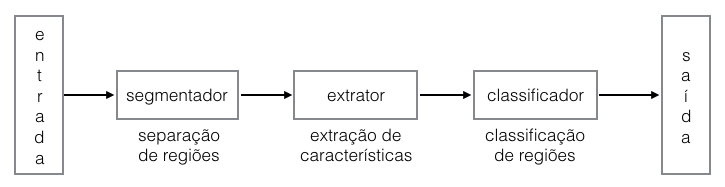
\includegraphics[width=\textwidth]{imgs/arquitetura_geral}
    \caption{Arquitetura geral da solução a ser desenvolvida para detecção de elementos antrópicos em imagens aéreas da floresta amazônica}
    \label{fig:metDiagramaGeral}
\end{figure}

A ideia geral é que imagens aéreas de regiões florestais da Amazônia legal sirvam de entrada para o problema. Estas mesmas imagens serão particionadas em regiões por um segmentador. Em seguida, um extrator será utilizado para criar o vetor de características de cada segmento provido pela etapa anterior. Por fim um classificador, composto por um ou mais algoritmos de classificação,  será utilizado para rotular as regiões com a finalidade de encontrar as regiões de elementos antrópicos. A saída do sistema pode, então, ser composta pelas regiões segmentadas e suas classificações finais.

Embora esta seja uma arquitetura simples, bastante difundida na literatura, nuances para o problema apresentado neste trabalho devem ser levadas em conta. Para chegarmos à conclusão de quais segmentadores, extratores e classificadores devem ser utilizados, são necessárias várias etapas de experimentação, validação de resultados e análises.

\section{Entrada}

Uma base de dados com imagens aéreas de floresta tropical precisa ser formada. Todas as imagens precisam ter as mesmas dimensões, condições visuais semelhantes e preferencialmente pertencerem à região de floresta amazônica, excluindo imagens de cidades e povoados da região.

Como serão processada por uma etapa de segmentação, as imagens não sofrerão nenhum tipo de filtragem, ficando estas a cargo dos segmentadores a serem avaliados. A base de imagens gerada nesta etapa é um dos objetivos específicos deste trabalho.

\section{Segmentador}\label{sec:metSegmentador}

Para encontrarmos o segmentador ideal, os métodos de segmentação de imagens considerados estado-da-arte serão aplicados à uma parte da base de imagens aéreas da floresta amazônica. Esta porção da base de imagens também será manualmente segmentada por seres humanos e servirá de base de comparação para a segmentação realizada pelos métodos experimentados. Ainda é preciso aferir a consistência da segmentação manual realizada por seres humanos. Métricas de erros de consistência como o \textit{Local Consistency Error} (LCE) e \textit{Global Consistency Error} (GCE) devem ser aplicados.

Esta etapa deve determinar o método de segmentação com melhores resultados, a ser utilizado na solução descrita pelo trabalho. A precisão e o tempo de execução devem ser utilizados para a avaliação do desempenho dos algoritmos testados. Em seguida, é preciso extrair as características dos segmentos gerados.

\section{Extrator}\label{sec:metExtrator}

Os algoritmos de classificação lidam com variáveis numéricas inteiras, de ponto flutuante e em alguns casos, dados textuais. No entanto, para classificar imagens, ou no caso deste trabalho, segmentos de imagens, é preciso que um conjunto de características seja extraído dos pixels destas imagens ou regiões e disponibilizados para o modelo de classificação.

Nesta etapa serão testadas diversas características disponíveis na literatura de processamento digital de imagens, especialmente informações sobre cor, intensidade, textura e morfologia destas amostras. Também deverão ser testadas técnicas para redução da dimensionalidade do vetor de amostras, tais quais técnicas que se utilizam de correlação e ganho de informação.

Como requisito da composição da base de dados de segmentos, bem como para avaliação e otimização do vetor de características, todas as amostras geradas pela etapa de segmentação devem ser rotuladas manualmente e contar com a avaliação de especialistas na inspeção deste tipo de imagem. Com a base devidamente criada e rotulada, experimentos para determinar os classificadores mais adequados podem ser feitos.

\section{Classificador}\label{sec:metClassificador}

Nesta etapa, quatro estratégias de classificação presentes na literatura serão abordadas. Elas não demandam alterações na arquitetura geral da solução, mas mudam a forma como a base é rotulada e organizada. As métricas de avaliação do aprendizado precisam ser ponderadas para cada estratégia.

É importante destacar que a classe de interesse, elementos antrópicos, permanece a mesma em todas as abordagens, e sua inspeção mais cuidadosa é vital na avaliação de todos os métodos utilizados.

\subsection{Classificador multi-classe}

Nesta estratégia, a base de segmentos gerada será rotulada entre cinco classes possíveis: floresta, vegetação rasteira, água, terra e elemento antrópico. Diversos algoritmos que possibilitam clasificação multi-classe serão utilizados, tendo em mente que é importante testar métodos simbólicos, bayesianos, não-paramétricos, máquina de vetores de suporte, entre outros.

Todos os métodos devem ser testados com a base completa de segmentos, mas também com a base pré-processada por um seletor de características, que será responsável pela redução do vetor de características do problema. Este detalhe do experimento servirá para determinar se a seleção de atributos nesta abordagem reduz a complexidade dos modelos gerados e o ruído na base de dados, possibilitando melhor taxa de aprendizagem.

Cada algoritmo deve ser responsável pela classificação de toda a base. Ao fim, métricas de aprendizado como acurácia, precisão e revocação serão utilizadas para comparar os métodos entre si.

\subsection{Classificador binário}

Neste experimento, a base de segmentos gerada será rotulada entre duas classes: elementos naturais e elementos antrópicos. A classe de elementos naturais agrupa o que originalmente seriam as classes de floresta, vegetação rasteira, água e terra.

Os classificadores utilizados serão os mesmos do experimento com classificadores multi-classe, visto que não há grande diferença metodológica nas duas abordagens. Todos os métodos também serão testados com seletores de características, e o impacto desta seleção também será avaliado.

Ao fim do experimento, as métricas propostas para o problema de aprendizado serão colhidas para cada método testado e utilizados para comparar os métodos entre si, bem como o impacto geral da seleção de atributos para esta abordagem.

\subsection{Classificador unário}

Assim como no experimento de classificadores binários, a base de dados de segmentos será dividida entre elementos naturais e elementos antrópicos, utilizando os mesmos critérios. À primeira vista, esta estratégia de aprendizado parece muito similar aos classificadores binários, mas a diferença está inicialmente nos algoritmos utilizados.

Como o aprendizado unário utiliza o conceito de classe majoritária e classe anômala (\textit{outlier}), é preciso definir que classes do problema exercerão estes papéis. Por uma simples questão de frequência estatística, fica definido que a classe de elementos naturais é a classe majoritária, enquanto a classe de elementos antrópicos é considerada a classe anômala.

Aqui também deve ser avaliado o impacto de um seletor de atributos aplicado ao vetor de características da base de dados, a fim de entender se há mudança significativa na taxa de aprendizado da classe anômala.

\subsection{Conjunto de classificadores unários}

Esta abordagem consiste na criação de modelos de aprendizado unários para cada classe do problema, exceto para a classe anômala. Sendo assim, um ou mais classificadores unários serão treinados para cada uma das classes de floresta, vegetação rasteira, água e terra.

A preparação da base de dados é um importante passo nesta estratégia de aprendizado, visto que diversas versões da base de segmentos terão de ser geradas, cada uma representando a classe não-anômala em questão como a classe majoritária e todas as demais como outliers.

O conjunto de classificadores criados serão agrupados em um \textit{ensemble} de classificadores e cada um dos modelos será utilizado na composição do veredito final, para a classificação da amostra. Diversas combinações de modelos e algoritmos deverão ser testadas, bem como diversas formas de combinar os resultados dos classificadores individuais.

Assim como todas as outras estratégias de classificação presentes neste trabalho, as métricas mais relevantes serão a acurácia, precisão e revocação da classe de interesse, de elementos antrópicos, que aqui é a classe anômala. As abordagens de classificação com melhor desempenho nestes quesitos ou mais promissoras devem ser apontadas ao fim destes experimentos.

\section{Saída}

 Os resultados dos experimentos anteriores devem sustentar a conclusão sobre quais métodos de segmentação e classificação são mais indicados para a solução. A saída da solução deve indicar quais segmentos da coleção de imagens original possuem elementos antrópicos. A avaliação do desempenho na detecção destes elementos é a métrica definitiva da adequação da solução para o problema proposto.

O próximo capítulo descreve os experimentos realizados e discute os resultados encontrados.